\PassOptionsToPackage{table}{xcolor}
\documentclass[svgnames]{beamer}
\usepackage{graphicx}
\usepackage{array}
\usepackage{textpos}
\usepackage{tcolorbox}
\usepackage{booktabs}
\usepackage{xcolor}
\usepackage{tikz}
\usepackage[makeroom]{cancel}
\usetikzlibrary{shapes,calc,matrix}

\usetheme{Boadilla}
\usecolortheme{dolphin}
\setbeamertemplate{navigation symbols}{}
\graphicspath{{fig/}}

\setbeamertemplate{itemize items}[default]
\setbeamertemplate{enumerate items}[default]
\setbeamertemplate{blocks}[default]
%\setbeamercolor{block body}{use={block body},bg=block body.bg!50!black}

\title[Entropy deposition in nuclear collisions]{Entropy deposition in ultra-relativistic \\ nucleus-nucleus collisions} 
\subtitle[Duke U.]{\vspace{0.2 in} \includegraphics[scale=0.25]{collision}}
\author[J. Scott Moreland]{} 
\date[\today]{} 

\newcommand{\trento}{T\raisebox{-.5ex}{R}ENTo}
\newcommand{\nch}{N_\text{ch}}

\begin{document}


%%%%%%%%%%%%%%%%%%%%%%%%%%%%%%%%%%%%%%%%%%%%%%%%%%%%%%%%%%%%%%%%%%%%%%%%%%%%%%%%%%%%%%%%%%%
\begin{frame}

\maketitle

\begin{textblock*}{2cm}(0.7cm,-1.8cm)
  \includegraphics[height=1.2cm]{logo}
\end{textblock*}

\begin{textblock*}{2cm}(9.9cm,-2.0cm)
  \includegraphics[height=1.6cm]{logo2}
\end{textblock*}

\begin{textblock*}{\linewidth}(0cm,-2.2cm)
  \centering
  J. Scott Moreland \\ Preliminary Exam \textbar ~\today \\ ~ 
  \\ \tiny Supported by NNSA Stewardship Science Graduate Fellowship
\end{textblock*}
  
\end{frame}

%%%%%%%%%%%%%%%%%%%%%%%%%%%%%%%%%%%%%%%%%%%%%%%%%%%%%%%%%%%%%%%%%%%%%%%%%%%%%%%%%%%%%%
{\setbeamercolor{background canvas}{bg=black}
\setbeamercolor{frametitle}{fg=white,bg=black}
\begin{frame}

 \frametitle{Early universe was \emph{extremely} hot and dense}
 
 \begin{center}
  \includegraphics[width=0.8\linewidth]{bigbang} \\
  \vspace{0.2 in}
  \textcolor{white}{$\lesssim 10^{-6}$ s after Big Bang temperatures exceeded \emph{trillions} of Kelvin} 
 \end{center}
 
\end{frame}}

%%%%%%%%%%%%%%%%%%%%%%%%%%%%%%%%%%%%%%%%%%%%%%%%%%%%%%%%%%%%%%%%%%%%%%%%%%%%
\begin{frame}

\frametitle{Primordial universe dominated by exotic state of matter}
\vspace{-0.05 in}

\begin{itemize}
 \item Quantum chromodynamics (QCD) predicts existence of new, exotic phase of matter at $T \gtrsim 10^{12}$ K which dominated the early universe \\
 \vspace{0.05 in}
 \item Under such conditions, hadronic states melt and form a deconfined soup of quarks and gluons known as \emph{quark-gluon plasma} (QGP)
\end{itemize}
\vspace{0.05 in}

\begin{columns}[T]
 \begin{column}{0.05\textwidth}
 \end{column}
 \begin{column}{0.45\textwidth}
  \centering
  \vspace{-0.05 in} \includegraphics[width=0.95\columnwidth]{confined_deconfined-crop} \\
 \end{column}
 \begin{column}{0.45\textwidth}
  \centering
  \includegraphics[width=0.8\columnwidth]{phasediagram1-crop}
  \vspace{0.05 in}
 \end{column}
 \begin{column}{0.05\textwidth}
 \end{column}
\end{columns}

\end{frame}

%%%%%%%%%%%%%%%%%%%%%%%%%%%%%%%%%%%%%%%%%%%%%%%%%%%%%%%%%%%%%%%%%%%%%%%%%%%%%%%%%%%%%%%%%%
\begin{frame}
 \frametitle{Creating quark-gluon plasma in the laboratory}
 
 \begin{columns}[T]
  \begin{column}{0.5\textwidth}
    \hrule
    \vspace{0.1 in}
    The predicted existence of a QGP phase of matter sparked a large scale effort to produce and study QGP in the laboratory. \\
    \vspace{0.1 in}
    This is accomplished by colliding heavy nuclei at ultra-relativistic energies $\sqrt{s} \sim 10-1000$ GeV
    \vspace{0.1 in}
    \hrule
  \end{column}
  \begin{column}{0.4\textwidth}
   \includegraphics[width=0.92\columnwidth]{phasediagram2-crop}
  \end{column}
 \end{columns}
 
 \centering
 \begin{textblock*}{\linewidth}(-5.15cm,0cm)
  \includegraphics[width=0.1\columnwidth]{arrow-crop}\vspace{0.5 in}
\end{textblock*}
 \hspace{0.3 in}
 \includegraphics[width=0.75\columnwidth]{hannah_collision.pdf} \\
 \vspace{-0.1 in} {\tiny ~~~~~FIG. by Hannah Petersen: picture of ultra-relativistic gold-gold collision}
\end{frame}


%%%%%%%%%%%%%%%%%%%%%%%%%%%%%%%%%%%%%%%%%%%%%%%%%%%%%%%%%%%%%%%%%%%%%%%%%%%%%%%%%%%%%%%%%%
\begin{frame}
\frametitle{Experimental effort to produce and study the QGP}

\begin{columns}[T]
 \begin{column}{0.5\textwidth}
  \centering
  {\small Relativistic Heavy-Ion Collider (RHIC)} \vspace{0.1 in}
  \includegraphics[width=0.8\columnwidth]{RHIC}
  \vspace{-0.2 in}
  \footnotesize
  \begin{itemize}
   \item Location: Brookhaven, NY
   \item Beam energies: $\sqrt{s} = 7.7 - 200$ GeV
   \item Detectors: STAR, PHENIX, PHOBOS, BRAHMS
   \item Projectiles: p+p, d+Au, Cu+Cu, Cu+Au, Au+Au, U+U, He$^3$-Au
  \end{itemize}
 \end{column}
 
 \vline \hspace{0.1 in}
 
 \begin{column}{0.5\textwidth}
  \centering
  {\small Large Hadron Collider (LHC)} \vspace{0.05 in}
  \includegraphics[width=0.9\columnwidth]{LHC}
  \vspace{0.05 in}
  \footnotesize
  \begin{itemize}
   \item Location: Geneva, Switzerland
   \item Beam energies: $\sqrt{s} = 2760$ GeV
   \item Detectors: ATLAS, ALICE, CMS
   \item Projectiles: p+p, p+Pb, Pb+Pb
  \end{itemize}
 \end{column}
 
\end{columns}
 
\end{frame}

%%%%%%%%%%%%%%%%%%%%%%%%%%%%%%%%%%%%%%%%%%%%%%%%%%%%%%%%%%%%%%%%%%%%%%%%%%%%%%%%%%%%%%%%%%%
\begin{frame}[t]{Surprising discovery, hot and dense QGP fireball flows!}
\vspace{0.1 in}
\begin{columns}
 \begin{column}{0.05\textwidth}
 \end{column}

 \begin{column}{0.3\textwidth}
  \centering
  \includegraphics[height=0.7\columnwidth]{collision1} \\
  \footnotesize elliptic fireball
 \end{column}
 
 \begin{column}{0.3\textwidth}
 \centering
  \hspace{0.15 in}
  \includegraphics[height=0.7\columnwidth]{collision2} \\
  \footnotesize elliptic pressure gradients
 \end{column}
 
 \begin{column}{0.3\textwidth}
  \centering
  \includegraphics[height=0.7\columnwidth]{collision22} \\
  \footnotesize elliptic final state
 \end{column}
 
 \begin{column}{0.05\textwidth}
 \end{column}
\end{columns}

\vspace{0.2 in}
\hrule
\vspace{0.2 in}

\centering
Similar elliptic flow phenonema has been observed in ultra-\emph{cold} atoms! \\
\vspace{0.05 in}
\includegraphics[width=0.9\textwidth]{ellipticflow2} \\
\vspace{0.05 in}
\footnotesize O'Hara, Hemmer, Gehm, Granade, Thomas, Science Dec 13 2002: 2179-2182 

\end{frame}

%%%%%%%%%%%%%%%%%%%%%%%%%%%%%%%%%%%%%%%%%%%%%%%%%%%%%%%%%%%%%%%%%%%%%%%%%%%%%%%%%%%%%%%%
\begin{frame}
  \frametitle{Flow evidenced by multi-particle correlations}

  \begin{columns}
  \begin{column}{0.6\textwidth}
  
  \begin{itemize}
    \footnotesize
    \item RHIC, LHC observe \emph{strong signals of collectivity}, i.e. particles emitted at similar angles detected with similar momenta.
    \vspace{0.1 in} \\
    \item Sinusoidal $\Delta \phi$ modulation consistent with emission from anisotropic momentum source. \emph{Evidence for flow!}
  \end{itemize}
  
  \vspace{0.15 in}
  \hrule
  \vspace{0.15 in}
  
  \begin{itemize}
    \footnotesize
    \item Azimuthal correlations characterized by their Fourier expansion, \\
    \begin{equation*}
    \frac{dN}{d\phi} \propto 1+\sum_n 2 v_n \cos n(\phi-\Psi_n)
    \end{equation*}
    \item Anisotropic flow coefficients $v_n$ quantify contribution from each harmonic.
  \end{itemize}
  
  \end{column}
  
  \begin{column}{0.4\textwidth}
    \vspace{0.15 in}
    \includegraphics[width=\columnwidth]{correlation_boxed}\\
    \vspace{0.1 in}
    \includegraphics[width=0.9\columnwidth]{harmonics}
  \end{column}
  \end{columns}
  
\end{frame}

%%%%%%%%%%%%%%%%%%%%%%%%%%%%%%%%%%%%%%%%%%%%%%%%%%%%%%%%%%%%%%%%%%%%%%%%%%%%%%
\begin{frame}

 \frametitle{Using hydrodynamics to model heavy-ion collisions}
 \vspace{0.05 in}
 \begin{columns}
  \begin{column}{0.4\textwidth}
   \vspace{0.15 in} \\
   \includegraphics[height=0.9\textheight]{evolution}
  \end{column}
  
  \begin{column}{0.5\textwidth}
  
  \begin{block}{\strut \small Initial conditions}
  \footnotesize Describe initial $T^{\mu\nu}$ at the QGP thermalization time 
  \end{block}
  
  \begin{block}{\strut \small Hydrodynamics (QGP)}
   \footnotesize Hydrodynamics imposes energy and momentum conservation, \\   
   \vspace{0.1 in}
   {\centering $\partial_\mu T^{\mu \nu} = 0$}\\
   \vspace{0.1 in}
   \footnotesize Equation of state from lattice QCD
  \end{block}

  \begin{block}{\strut \small Boltzmann Eqn (hadron gas)}
    \footnotesize Fluid discretized into particles. Non-equillibrium Boltz. transport,
    \vspace{0.1 in} \\
    \centering
    $\frac{df_i(x,p)}{dt} = \mathcal{C}_i(x,p)$ 
  \end{block}
  
  \vspace{0.2 in}

  \end{column}
  \end{columns}

 
\end{frame}

%%%%%%%%%%%%%%%%%%%%%%%%%%%%%%%%%%%%%%%%%%%%%%%%%%%%%%%%%%%%%%%%%%%%%
\begin{frame}
  \includegraphics[width=\textwidth]{model-to-data}
\end{frame}


%%%%%%%%%%%%%%%%%%%%%%%%%%%%%%%%%%%%%%%%%%%%%%%%%%%%%%%%%%%%%%%%%%%%%%%%%%%%%%%%%%%%%
\begin{frame}{Underconstrained parameters: the QGP shear viscosity}

\begin{columns}
 \begin{column}{0.55\textwidth}
  \begin{itemize}
    \item Shear viscosity $\eta$ quantifies fluid's resistance to shearing flows
    \vspace{0.05 in}
    \item Shear stress $\tau = \eta \frac{dv}{dy}$
  \end{itemize}
 \end{column}
 \begin{column}{0.35\textwidth}
  \vspace{0.1 in} \includegraphics[width=\columnwidth]{shearflow-crop}
 \end{column}
 \begin{column}{0.1\textwidth}
 \end{column}
\end{columns}
\vspace{0.2 in}
\centering Scaled by entropy density to form dimensionless viscosity measure \textcolor{red}{$\eta/s$}
\vspace{0.1 in}
\begin{columns}
 \begin{column}{0.5\textwidth}
  \includegraphics[width=\columnwidth]{ellipticflow_viscous}
    \begin{textblock*}{\linewidth}(3.cm,-3.4cm)
      \footnotesize
      small $\eta/s$ \\
      large $v_2$
    \end{textblock*}
    \begin{textblock*}{\linewidth}(3.cm,-1.1cm)
      \footnotesize
      large $\eta/s$ \\
      small $v_2$
    \end{textblock*}
 \end{column}
 
 \begin{column}{0.5\textwidth}
  \centering \vspace{0.15 in}
  \includegraphics[width=\columnwidth]{three} \\
  \tiny Schenke, Jeon, Gale Phys. Rev. Lett. 106, 042301
 \end{column}
\end{columns}
\vspace{0.1 in}
\begin{columns}
 \begin{column}{0.5\textwidth}
  \centering suppresses flow anisotropy
 \end{column}
 \begin{column}{0.5\textwidth}
  \centering washes out small structures
 \end{column}

\end{columns}
 
\end{frame}

%%%%%%%%%%%%%%%%%%%%%%%%%%%%%%%%%%%%%%%%%%%%%%%%%%%%%%%%%%%%%%%%%%%%%%%%%%%%%%%%%%%%%%%%%%%%
\begin{frame}[t,noframenumbering]{Harmonic decomposition of anisotropic flow}
\vspace{0.1 in}
\begin{columns}
 \begin{column}{0.05\textwidth}
 \end{column}

 \begin{column}{0.3\textwidth}
  \centering
  \includegraphics[height=0.7\columnwidth]{collision1} \\
  \footnotesize elliptic fireball
 \end{column}
 
 \begin{column}{0.3\textwidth}
 \centering
  \hspace{0.15 in}
  \includegraphics[height=0.7\columnwidth]{collision2} \\
  \footnotesize elliptic pressure gradients
 \end{column}
 
 \begin{column}{0.3\textwidth}
  \centering
  \includegraphics[height=0.7\columnwidth]{collision22} \\
  \footnotesize elliptic final state
 \end{column}
 
 \begin{column}{0.05\textwidth}
 \end{column}
\end{columns}

\vspace{0.2 in}
\hrule
\vspace{0.2 in}

\begin{columns}
 \begin{column}{0.05\textwidth}
 \end{column}

 \begin{column}{0.3\textwidth}
  \centering
  \includegraphics[height=0.7\columnwidth]{collision3} \\
  \footnotesize triangular fireball
 \end{column}
 
 \begin{column}{0.3\textwidth}
 \centering
  \hspace{0.15 in}
  \includegraphics[height=0.7\columnwidth]{collision4} \\
  \footnotesize triangular pressure gradients
 \end{column}
 
 \begin{column}{0.3\textwidth}
  \centering
  \includegraphics[height=0.7\columnwidth]{collision44} \\
  \footnotesize triangular final state
 \end{column}
 
 \begin{column}{0.05\textwidth}
 \end{column}
\end{columns}

\end{frame}

%%%%%%%%%%%%%%%%%%%%%%%%%%%%%%%%%%%%%%%%%%%%%%%%%%%%%%%%%%%%%%%%%%%%%%%%%%%%%%%%%%%
\begin{frame}{Extracting $\eta/s$ from model to data comparison}
\vspace{0.15 in}
\centering \includegraphics[width=0.9\columnwidth]{conversion-crop}

 \begin{textblock*}{\linewidth}(-1.7cm,0.06cm)
  \centering
  \small
  $\varepsilon_n = \left |\frac{\int dx \, dy\, r^n e^{i n \phi} \, s(x,y)}{\int dx \, dy \, r^n \, s(x,y)} \right|$
\end{textblock*}

\begin{textblock*}{\linewidth}(3.4cm,0.2 cm)
  \centering
  \small
  $v_n(p_T,y)  = \langle \langle \cos[n(\phi-\Psi_n)] \rangle \rangle$
\end{textblock*}
\vspace{0.1 in}
\begin{columns}
 \begin{column}{0.75\textwidth}
  \begin{block}{\vspace*{-3ex}}
    \centering
    $\eta/s$ moderates conversion rate: $\varepsilon_n \rightarrow v_n$ \\ 
    \vspace{0.05 in}
    value extracted by tuning $\eta/s$ to fit observed $v_n$
  \end{block}
 \end{column}
\end{columns}

\end{frame}

%%%%%%%%%%%%%%%%%%%%%%%%%%%%%%%%%%%%%%%%%%%%%%%%%%%%%%%%%%%%%%
\begin{frame}{Simulations indicate QGP nearly inviscid!}

 \begin{columns}
 \begin{column}{0.45\columnwidth}
 \centering
 \includegraphics[width=\columnwidth]{bjorn}
 \end{column}
 \begin{column}{0.55\columnwidth}
 \centering
 \vspace{0.05 in} \includegraphics[width=\columnwidth]{eta-bound}
 \end{column}
 \end{columns}
 
 \begin{columns}
 \begin{column}{0.45\columnwidth}
 \centering
 \tiny Gale, Jeon, Schenke, Tribedy, Phys.Rev.Lett. 110 (2013)
 \end{column}
 \begin{column}{0.55\columnwidth}
 \centering
 \tiny A Adams, et. al. New Journal of Physics 14 (2012)
 \end{column}
 \end{columns}
 
 \vspace{0.1 in}
 
\begin{itemize}
  \item Left: QGP specific shear viscosity $\eta/s$ tuned to fit experimental flows
  \item Right: $\eta/s$ temp. dependence compared for several notable fluids
\end{itemize}
\vspace{-0.2 in}
\begin{columns}
 \begin{column}{0.78\textwidth}
  \begin{block}{\vspace*{-3ex}}
  \centering 
    Conservative estimates place $(\eta/s)_\text{QGP} \sim 0.08$ - $0.2$ \\ 
    \vspace{0.05 in}
    Can we improve this uncertainty to $\mathcal{O}(20\%)$?
 \end{block}
 \end{column}

\end{columns}
\end{frame}


%%%%%%%%%%%%%%%%%%%%%%%%%%%%%%%%%%%%%%%%%%%%%%%%%%%%%%%%%%%%%%%%%%%%%%%%%%
\begin{frame}
 \centering
 \vspace{-1 in}
 \includegraphics[width=0.8\columnwidth]{initialconditions}
 
 \begin{textblock*}{0.7\linewidth}(2cm,-3cm)
  \begin{itemize}
   \item Generate profiles of entropy (energy) at the QGP thermalization time
   \begin{equation*}
    \frac{dS(\vec{x})}{dy} \bigg \vert_{\tau = \tau_\text{therm}}
   \end{equation*}
  \item $dS/dy$ and equation of state initialize $T^{\mu\nu}$
  \item Hydrodynamics evolves system forward in time 
  \begin{equation*}
   \partial_\mu T^{\mu \nu} = 0
  \end{equation*}

  \end{itemize}
 \end{textblock*}
\end{frame}

%%%%%%%%%%%%%%%%%%%%%%%%%%%%%%%%%%%%%%%%%%%%%%%%%%%%%%%%%%%%%%%%%%%%%%%%%%%%
\begin{frame}{Analytical Glauber model}

  \begin{columns}
  
   \begin{column}{0.5\textwidth}
   \centering
   \vspace{0.1 in} \tiny Miller, et. al., Ann.Rev.Nucl.Part.Sci.57:205-243 (2007) \\
   \includegraphics[width=\textwidth]{glauber}
   \end{column}
  
   \begin{column}{0.5\textwidth}
   
    \begin{enumerate}
      \small \item Parameterize nuclear density
    \end{enumerate}
   \vspace{-0.025 in}
   \begin{equation*}
    \rho(r) = \frac{\rho_0}{1+\exp(\tfrac{r-R}{d})}
   \end{equation*}
   
   \begin{enumerate}
   \setcounter{enumi}{1}
    \small \item Flatten density along beam dim.
   \end{enumerate}
   \vspace{-0.025 in}
   \begin{equation*}
    T_{A,B}(x,y) = \int dz\, \rho_{A,B}(x,y,z)
   \end{equation*}
  
  \end{column}
  \end{columns}
   
  \begin{enumerate}
  \setcounter{enumi}{2}
    \small \item Nucleon participant density (wounded nucleons) 
  \end{enumerate}
  \vspace{-0.05 in}
  $\overline{\text{WN}}(x,y; b) = T_A(x+b/2,y)\left(1-\left(1-\sigma_\text{NN}^\text{inel} T_B(x-b/2,y)/B \right)^B \right) + ...$
  \vspace{0.1 in}
  \begin{enumerate}
    \setcounter{enumi}{3}
    \small \item Nucleon-nucleon collision density (binary collisions) 
  \end{enumerate}
  \vspace{0.025 in}
  $\overline{\text{BC}}(x,y; b) = \sigma_\text{NN}^\text{inel} T_A(x+b/2,y)  T_B(x-b/2,y)$
  
  \begin{block}{\vspace*{-3ex}}
   \centering
   Two-component ansatz:~~ $\frac{dS}{dy} \big \vert_{y=0} \propto \frac{1-\alpha}{2}\, \overline{\text{WN}} + \alpha\, \overline{\text{BC}}$
  \end{block}

\end{frame}

%%%%%%%%%%%%%%%%%%%%%%%%%%%%%%%%%%%%%%%%%%%%%%%%%%%%%%%%%%%%%%%%
\begin{frame}{Monte Carlo Glauber model}
 \begin{columns}[T]
  \begin{column}{0.5\textwidth}
   \begin{itemize}
    \item Smooth nuclear density replaced with discrete nucleon config's
    \vspace{0.1 in}
    \item Nucleon-nucleon collisions calculated \emph{stochastically},
    \begin{equation}
    \small
    P_\text{coll}=
    \begin{cases}
    1 &\mbox{if } b^2 \le \sigma^\text{inel}_\text{NN}/\pi \\ 
    0 &\mbox{if } b^2 > \sigma^\text{inel}_\text{NN}/\pi, \nonumber
    \end{cases}
    \end{equation}
   \end{itemize}
  \end{column}
  
  \begin{column}{0.5\textwidth}
   \centering
   \vspace{-0.1 in}
   \includegraphics[width=0.8\columnwidth]{toyglauber8-crop} \\
   \footnotesize Pb-Pb participants (red) $b=8$ fm
  \end{column}

 \end{columns}

 \vspace{0.1 in}
 
 \begin{columns}[T]
  \begin{column}{0.5\textwidth}
   \begin{itemize}
    \item Same two-component ansatz,\\
    \vspace{0.1 in}
    $\frac{dS}{dy} \big \vert_{y=0} \propto \frac{1-\alpha}{2}\, \text{WN} + \alpha\, \text{BC}$
    \vspace{0.1 in}
    \item Nucleon fluctuations explained existence of odd flow harmonics!
   \end{itemize}
   \centering
   \vspace{0.05 in}
   \footnotesize FIG. Chun Shen, Ph.D. Thesis
  \end{column}
  \begin{column}{0.5\textwidth}
  \centering
  \vspace{0.1 in}
  \includegraphics[width=0.8\columnwidth]{chun_glb_thesis} 
  \end{column}
 \end{columns}

\end{frame}

%%%%%%%%%%%%%%%%%%%%%%%%%%%%%%%%%%%%%%%%%%%%%%%%%%%%%%%%%%%%%%%%%%%%%%%%%%%%
\begin{frame}{Color Glass Condensate (CGC) theory}

\begin{columns}
 \begin{column}{0.6\textwidth}
  \begin{itemize}
  \item Proton structure dominated by soft gluons at high energy
  \item Gluon density eventually saturates and preserves finite proton cross section
  \item Saturation characterized by intrinsic momentum scale $Q_s$ [GeV]
  \item Occupation of gluons larger than $1/Q_s$ is suppressed
 \end{itemize}
 \end{column}
 \begin{column}{0.4\textwidth}
  \centering
  \includegraphics[width=\columnwidth]{PDF} \\
  \tiny \vspace{-0.05 in}
  ~~Nucl.Phys.Proc.Suppl. 191 (2009) 5-15\\
  \vspace{0.05 in}
  ~~x denotes fraction of proton momentum
  
 \end{column}
\end{columns}

 \centering
 \vspace{0.15 in}
 \includegraphics[width=0.5\columnwidth]{CGC-crop} 
\end{frame}

%%%%%%%%%%%%%%%%%%%%%%%%%%%%%%%%%%%%%%%%%%%%%%%%%%%%%%%%%%%%%%%%%%%%%%%%%
\begin{frame}[t]{The CGC-based IP-Glasma model}
{\centering Schenke, Tribedy, Venugopalan, Phys.Rev.\ C86 (2012) 034908}
  
  \begin{columns}[T]
   \begin{column}{0.6\textwidth}
    \begin{enumerate}
      \item Initial-state quantum fluctuations of nucleon positions and sub-nucleonic color charges (including saturation)
      \vspace{0.2 in}
      \item Generate color fields from underlying charge distribution
      \vspace{0.2 in}
      \item Evolve initial energy-momentum tensor by solving weakly-coupled (2+1)-dim. Yang-Mills equations $[D_\mu,F^{\mu\nu}] = J^\nu$
      \vspace{0.2 in}
      \item Match energy-momentum tensor to hydrodynamic simulations at $\tau_{therm}$
    \end{enumerate}
   \end{column}
   
   \begin{column}{0.4\textwidth}
    \centering
    \vspace{-0.1 in}
    \includegraphics[width=0.8\columnwidth]{initial_nuclei}\\
    \includegraphics[width=0.8\columnwidth]{gluonfields} \\
    \vspace{0.1 in}
    \includegraphics[width=0.8\columnwidth]{ipglasma_event}
   \end{column}

  \end{columns}
  
\end{frame}

%%%%%%%%%%%%%%%%%%%%%%%%%%%%%%%%%%%%%%%%%%%%%%%%%%%%%%%%%%%%%%%%%%%%%%
\begin{frame}{IP-Glasma model: important results}
 \begin{columns}
  \begin{column}{0.5\textwidth}
   \centering
   \begin{itemize}
    \item Excellent description of heavy-ion flows 
    \vspace{0.1 in}
    \item Correct event-by-event flow fluctuations
   \end{itemize}
   \vspace{0.2 in}
   \includegraphics[width=\columnwidth]{Glasma_flows}
  \end{column}
  
  \begin{column}{0.5\textwidth}
   \centering
   \includegraphics[width=0.85\columnwidth]{Glasma_fluctuations} \\
   \tiny Schenke et al. Nucl.Phys. A926 (2014) 102-108
  \end{column}

 \end{columns}
\end{frame}

\begin{frame}{Examples where existing models fail}

 {\large MC-Glauber}
 \begin{itemize}
  \item Binary collision scaling is inconsistent with recent Uranium-Uranium data from STAR (somewhat technical, more on this later)
  \begin{equation*}
   \frac{dS}{dy} \big \vert_{y=0} \propto \frac{1-\alpha}{2}\, \overline{\text{WN}} + \xcancel{ \alpha\, \overline{\text{BC}}}
  \end{equation*}

 \end{itemize}
 
 {\large IP-Glasma}
 \begin{itemize}
   \item Cannot simulate small systems without changing model parameters
   \vspace{0.1 in}
   \item Model gives poor description of p+p, p+Pb multiplicity distributions
 \end{itemize}
\end{frame}

%%%%%%%%%%%%%%%%%%%%%%%%%%%%%%%%%%%%%%%%%%%%%%%%%%%%%%%%%%%%%%%%%%%
\begin{frame}{Case for new initial condition models}
\vspace{0.15 in}
\begin{itemize}
 \item MC-Glauber model all but killed off by recent U+U results
 \vspace{0.1 in}
 \item IP-Glasma, while highly successful in heavy-ion collisions, \\struggles for small collision systems
\end{itemize}
\vspace{0.1 in}
\begin{columns}
 \begin{column}{0.85\textwidth}
   \emph{
   As community turns attention to exciting new results for p+Pb, d+Au and He$^3$+Au collisions which indicate QGP production in small systems, there is a clear need
   for initial condition models which unite small and large collisions under a single framework}
 \end{column}
\end{columns}

\centering
\vspace{0.1 in}
\includegraphics[width=0.6\columnwidth]{validity-crop}
\vspace{0.1 in}
\end{frame}

\begin{frame}
 \centering
 \includegraphics[width=0.8\columnwidth]{trentoheader}
\end{frame}

%%%%%%%%%%%%%%%%%%%%%%%%%%%%%%%%%%%%%%%%%%%%%%%%%%%%%%%%%%%%%%%%%%%%%%%%%%%%%%%%%%%%%%%%%%%
\begin{frame}
  \frametitle{Entropy deposition in nuclear collisions as a mapping}
  
  \begin{enumerate}
   \item Factorization: nuclear collision $\rightarrow$ sum local nucleon collisions
   \item Consider entropy deposited by all possible m-on-n nucleon collisions
  \end{enumerate}
  
  \vspace{0.1 in}
  
  \begin{columns}
   \begin{column}{0.5\textwidth}
    \centering
    \includegraphics[width=0.55\columnwidth]{motivation1-crop} \\
    \includegraphics[width=0.55\columnwidth]{motivation2-crop}
   \end{column}
   \begin{column}{0.5\textwidth}
     \flushleft
     \vspace{0.05 in}
     \includegraphics[width=0.9\columnwidth]{TATB_diagram1-crop}
   \end{column}
  \end{columns}
  
  \begin{textblock*}{2cm}(5cm,-1.15cm)
    \includegraphics[scale=0.2]{arrowz-crop}
  \end{textblock*}
  
  \vspace{0.1 in}
  
  \begin{enumerate}
  \setcounter{enumi}{2}
   \item Taking cell size to zero, defines a mapping $dS/d^2r \equiv f(T_A,T_B)$
  \end{enumerate}
  \centering
  Fundamental assumption: \emph{early time entropy deposition is local}
\end{frame}

%%%%%%%%%%%%%%%%%%%%%%%%%%%%%%%%%%%%%%%%%%%%%%%%%%%%%%%%%%%%%%%%%%%%%%%%%%%%%%%%%%%%%%%%%%%%%
\begin{frame}[t]{Constructing a suitable ansatz for entropy deposition}
\emph{what limits/constraints must the mapping f obey?}

\vspace{0.2 in}
\begin{columns}
\begin{column}{0.9\textwidth}
\underline{Fundamental constraints}
\vspace{0.05 in}
\begin{itemize}
 \item Symmetric function of $T_A$ and $T_B$
 \item Monotonically increasing with respect to $T_A$, $T_B$
\end{itemize}
\vspace{0.1 in}
\underline{Empirical constraints}
\vspace{0.05 in}
\begin{itemize}
 \item $f(T,T) \propto T$  \\
 %\footnotesize (e.g. ratio $dN/d\eta$ central $\text{Au}^{197}$+$\text{Au}^{197}$ vs $\text{Cu}^{63}+\text{Cu}^{63}$ is $\sim N_\text{part}^\text{Au+Au}:N_\text{part}^\text{Cu+Cu}$)
\end{itemize}
\vspace{0.1 in}
\underline{Limiting cases}
\vspace{0.05 in}
\begin{itemize}
 \item If either $T_A$, $T_B$ goes to zero, $f(T_A,T_B)$ goes to zero
 \item Asymmetric collisions $T_A \ne T_B$ characterized by two scales: \\ $\min(T_A,T_B)$ and $\max(T_A,T_B)$
\end{itemize}
\end{column}

\end{columns}

\end{frame}

%%%%%%%%%%%%%%%%%%%%%%%%%%%%%%%%%%%%%%%%%%%%%%%%%%%%%%%%%%%%%%%%%%%%%%%%%%%%%%%%%%%%%%%%%
\begin{frame}{Constructing a suitable ansatz for entropy deposition}

\begin{equation}
 f \equiv M(p;T_A,T_B) = \left(\frac{T_A^p + T_B^p}{2} \right) ^{1/p} \nonumber
\end{equation}
Dimensionless parameter $p$ smoothly interpolates space of vector two-norms, e.g.
\begin{equation}
  M(p; T_A, T_B) =
  \begin{cases}
    \dfrac{2\, T_A T_B}{T_A + T_B} & p = -1 \text{ (harmonic mean)}, \\[2ex]
    \sqrt{T_A T_B} & p = 0 \text{ (geometric mean)}, \\[2ex]
    \dfrac{T_A + T_B}{2} & p = 1 \text{ (arithmetic mean)}, \\[2ex]
  \end{cases}
  \nonumber
\end{equation}
and assumes the limiting values
\begin{eqnarray}
 \lim\limits_{p\rightarrow -\infty}M(p;T_A,T_B) \rightarrow \min{(T_A,T_B)}, \nonumber \\
 \lim\limits_{p\rightarrow \infty}M(p;T_A,T_B) \rightarrow \max{(T_A,T_B)}. \nonumber
\end{eqnarray}
 
\end{frame}

%%%%%%%%%%%%%%%%%%%%%%%%%%%%%%%%%%%%%%%%%%%%%%%%%%%%%%%%%%%%%%%%%%%%%%%%%%%%%%%%%%%%%%%%%
\begin{frame}{Comparing {\trento} ansatz to MC-Glauber ansatz}

\begin{columns}[T]

 \begin{column}{0.5\textwidth}
  \centering
  MC-Glauber (two-component):\\
  \vspace{0.05 in}
  $f \sim (1-\alpha) (T_A+T_B) + \alpha\, T_A\,T_B$ \\
  \vspace{0.2 in}
  {\trento} (generalized mean): \\
  \vspace{0.05 in}
  $f \sim \left(\frac{T_A^p + T_B^p}{2} \right) ^{1/p}$
 \end{column}
 
 \begin{column}{0.45\textwidth}
  \centering
  \includegraphics[width=0.7\columnwidth]{TATB_diagram-crop}
 \end{column}
 
 \begin{column}{0.1 in}
 \end{column}
\end{columns}

\vspace{0.3 in}

\underline{Models deviate from canonical participant scaling in distinct ways}
\begin{itemize}
 \vspace{0.1 in}
 \item MC-Glauber: modifies \emph{symmetric} deposition $T_A \approx T_B$
 \vspace{0.1 in}
 \item \trento: modifies \emph{asymmetric} deposition $T_\text{min} \ll T_\text{max}$ 
\end{itemize}

\end{frame}

%%%%%%%%%%%%%%%%%%%%%%%%%%%%%%%%%%%%%%%%%%%%%%%%%%%%%%%%%%%%%%%%%%%%%%%%%%%%%%%%%%%%%%%%%%%%%%%%%%%%%%%%%%
\begin{frame}{Comparing {\trento} ansatz to MC-Glauber ansatz}
 \includegraphics[width=\columnwidth]{comparison}
\end{frame}

%%%%%%%%%%%%%%%%%%%%%%%%%%%%%%%%%%%%%%%%%%%%%%%%%%%%%%%%%%%%%%%%%%%%%%%%%%%%%%%%%%%%%%%%%%%%%%%%%%%%%%%%
\begin{frame}{{\trento}: new model for ultra-relativistic nuclear collisions}
\vspace{0.1 in}
\begin{columns}
 \begin{column}{0.6\textwidth}
 \begin{enumerate}
  \item Sample MC nucleon configurations for projectile and target nuclei
 \end{enumerate}
 \end{column}
 \begin{column}{0.4\textwidth}
  \hspace{0.2 in} \vspace{-0.2 in} \includegraphics[width=0.6\columnwidth]{evolution1}
 \end{column}
\end{columns}
\vspace{0.2 in}
\begin{enumerate}
\setcounter{enumi}{1}
\item Calculate nucleon participants using a probabilistic collision criteria
  \begin{equation}
  P_\text{coll} = 1 - \exp \left[ -\sigma_\text{gg} \int dx\, dy \int dz\, \rho_A \int dz\, \rho_B \right], \nonumber
  \end{equation}
  \begin{center}
    \includegraphics[width=0.5\columnwidth]{protonproton-crop}
  \end{center}
\end{enumerate}

\end{frame}

%%%%%%%%%%%%%%%%%%%%%%%%%%%%%%%%%%%%%%%%%%%%%%%%%%%%%%%%%%%%%%%%%%%%%%%%%%%%%%%%%%%%%%%%%%%%%%%
\begin{frame}{{\trento}: new model for ultra-relativistic nuclear collisions}
\vspace{0.15 in}
 \begin{columns}
 \begin{column}{0.6\textwidth}
  \begin{enumerate}
  \setcounter{enumi}{2}
   \item Calculate \emph{fluctuated} nuclear thickness functions $T_A$, $T_B$ for each nucleus
   {\footnotesize
  \begin{equation}
  T_{A}(x,y) = \sum\limits_i \gamma_i \int dz\, \rho_{A}(x-x_i,y-y_i,z-z_i), \nonumber
  \end{equation}}
  $\gamma_i$ sampled from Gamma distribution with unit mean and shape parameter $k$. Encodes min-bias p+p fluctuations.
  \end{enumerate}
 \vspace{0.1 in}
 \end{column}
 \begin{column}{0.4\textwidth}
 \centering
 \includegraphics[width=0.7\columnwidth]{TA2}
 \end{column}
 \end{columns}
 
\begin{enumerate}
  \setcounter{enumi}{3}
  \item Generate ``reduced thickness'' using generalized mean
  \begin{equation}
    T_R(p;T_A,T_B) \equiv \left(\frac{T_A^p + T_B^p}{2} \right) ^{1/p} \nonumber
  \end{equation}
 
  \item Entropy density at mid-rapidity set proportional to $T_R$
  \begin{equation}
  \frac{dS(x,y)}{d^2r_\perp d\eta} \bigg \vert_{\eta=0} \propto T_R(p;x,y) \nonumber
  \end{equation}

\end{enumerate}

\end{frame}

%%%%%%%%%%%%%%%%%%%%%%%%%%%%%%%%%%%%%%%%%%%%%%%%%%%%%%%%%%%%%%%%%%%%%%%%%%%%%%%%%%%%%%%%%%%%%%%%%%%%%%%%%%%
\begin{frame}{Example {\trento} events}
\centering
\includegraphics[width=0.9\columnwidth]{trento-profiles} \\
Transverse entropy density for two random Pb+Pb \\ events calculated using $p=0$ (geometric mean)
\end{frame}

%%%%%%%%%%%%%%%%%%%%%%%%%%%%%%%%%%%%%%%%%%%%%%%%%%%%%%%%%%%%%%%%%%%%%%%%%%%%%%%%%%%%%%%%%%%%%%%%%%%%%%%%%%
\begin{frame}[t]{Results: multiplicity distributions}
 \vspace{0.2 in}
 \setlength{\leftmargini}{30pt}
 \includegraphics[width=\columnwidth]{multdist}
 
 \begin{textblock*}{0.65\textwidth}(4.25cm,-4cm)
  \textblockcolor{white}
  \vspace{0.2 in}
  
  {\hspace{-0.1 in} \large $\leftarrow$ Tune free parameters to fit p+p collisions}\\
  \begin{enumerate}
   \normalsize
   \item Overall norm, $dN_\text{ch}/dy \propto \int dx dy T_R(x,y)$
   \item Gamma fluctuation factor $k=1.25$
   \item Generalized mean parameter $p=0$
   \item Nucleon width $\sigma_N=0.6$ fm (insensitive)
  \end{enumerate}
 
 \vspace{1.25 in}
 \end{textblock*}
 
 \begin{itemize}
  \item {\trento} results (solid lines) plotted against ALICE data (symbols)
 \end{itemize}
\end{frame}

\begin{frame}[t,noframenumbering]{Results: multiplicity distributions}
 \vspace{0.2 in}
 \includegraphics[width=\columnwidth]{multdist}
 \begin{itemize}
  \item {\trento} results (solid lines) plotted against ALICE data (symbols)
  \vspace{0.05 in}
  \item p+p and p+Pb distributions emerge naturally!
 \end{itemize}
 
  \hspace{4 in}
 \begin{textblock*}{0.33\textwidth}(8.3cm,-6.25cm)
 \textblockcolor{white}
 ~\vspace{1.75 in}
 \end{textblock*}
\end{frame}

\begin{frame}[t,noframenumbering]{Results: multiplicity distributions}
 \vspace{0.2 in}
 \includegraphics[width=\columnwidth]{multdist}
  \begin{itemize}
  \item {\trento} results (solid lines) plotted against ALICE data (symbols)
  \vspace{0.05 in}
  \item p+p and p+Pb distributions emerge naturally!
  \vspace{0.05 in}
  \item Small variances in normalization consistent with variances in kinematic cuts and beam energies 
 \end{itemize}
\end{frame}

\begin{frame}[t,noframenumbering]{Results: multiplicity distributions}
 \vspace{0.2 in}
 \includegraphics[width=\columnwidth]{multdist}
  \begin{itemize}
  \item {\trento} results (solid lines) plotted against ALICE data (symbols)
  \vspace{0.05 in}
  \item p+p and p+Pb distributions emerge naturally!
  \vspace{0.05 in}
  \item Small variances in normalization consistent with variances in kinematic cuts and beam energies 
 \end{itemize}
\end{frame}

\begin{frame}[t,noframenumbering]{Results: multiplicity distributions}
 \vspace{0.2 in}
 \includegraphics[width=\columnwidth]{multdist}
 \begin{columns}[T]
  \begin{column}{0.7\textwidth}
   \centering
   \includegraphics[width=\columnwidth]{Glasma_pp_pA} \\
   \vspace{0.1 in}
   \scriptsize Schenke et al. Nucl.Phys. A926 (2014) 
  \end{column}
   \begin{column}{0.3\textwidth}
   \vspace{0.1 in}
   $\leftarrow$ IP-Glasma p+p and p+Pb results with additional fluctuations added (red)
  \end{column}
 \end{columns}
 

\end{frame}

%%%%%%%%%%%%%%%%%%%%%%%%%%%%%%%%%%%%%%%%%%%%%%%%%%%%%%%%%%%%%%%%%%%%%%%%%%%%%%%%%%%%%%%%%%%%%%%%%%%%%%%
\begin{frame}{Results: eccentricity harmonics}
 \centering
 \begin{itemize}
  \item Eccentricity $\varepsilon_n$ quantifies magnitude of each harmonic \\
	 $\varepsilon_2 \leftrightarrow$ ellipticity, $\varepsilon_3 \leftrightarrow$ triangularity, etc
  \vspace{0.1 in}
  \item Formal definition: $\varepsilon_n = \left |\frac{\int dx \, dy\, r^n e^{i n \phi} \, s(x,y)}{\int dx \, dy \, r^n \, s(x,y)} \right|$
  \vspace{0.1 in}
  \item Models with larger eccentricities $\varepsilon_n$ require larger $\eta/s$ to fit observed anisotropic flow $v_n$. 
	Crucial that model predicts acccurate $\varepsilon_n$ coeff's!
 \end{itemize}
 \vspace{0.1 in}
 \includegraphics[width=0.8\columnwidth]{eccentricity2}\\
 \vspace{0.1 in}
 \scriptsize Centrality: fraction of total events ordered by multiplicity, $0\% \leftrightarrow$ highest multiplicity

 \begin{textblock*}{0.05\textwidth}(3.4cm,-2cm)
  \small Pb+Pb
 \end{textblock*}
\end{frame}

%%%%%%%%%%%%%%%%%%%%%%%%%%%%%%%%%%%%%%%%%%%%%%%%%%%%%%%%%%%%%%%%%%%%%%%%%%%%%%
\begin{frame}{Results: eccentricity harmonics}
 \centering
 \begin{itemize}
  \item Anisotropic flow data constrains allowable values of $\varepsilon_2$, $\varepsilon_3$ ratio,
  \begin{equation*} 
    \text{Ratio} = \sqrt{\langle \varepsilon_2^2 \rangle} / \sqrt{\langle \varepsilon_3^2 \rangle}^{0.6}
  \end{equation*}
  
  \item Left: Different initial condition models plotted against experimentally allowed region (grey band)
  \vspace{0.05 in}
  \item Right: {\trento} results show geometric mean $p=0$ tracks 
        $\varepsilon_2$ and $\varepsilon_3$ ratio compatible with LHC data.
 \end{itemize}
 \begin{columns}
  \begin{column}{0.5\textwidth}
   \centering
   \includegraphics[width=\columnwidth]{LHC_flow} \\
   \centering \tiny Retinskaya, Luzum \& Ollitrault: NP A926 (2014) 152-158
  \end{column}
  \begin{column}{0.5\textwidth}
   \centering
   \vspace{-0.05 in}\\
   \includegraphics[width=0.82\columnwidth]{vn_ratio-crop}
  \end{column}
 \end{columns}

 \begin{textblock*}{0.05\textwidth}(6.1cm,-3.3cm)
  \tiny \rotatebox{90}{$\sqrt{\langle \varepsilon_2^2 \rangle} / \sqrt{\langle \varepsilon_3^2 \rangle}^{0.6}$}
 \end{textblock*}
 
\end{frame}

%%%%%%%%%%%%%%%%%%%%%%%%%%%%%%%%%%%%%%%%%%%%%%%%%%%%%%%%%%%%%%%%%%%%%%%%%
\begin{frame}[fragile]{Results: Uranium-Uranium collisions}
 \vspace{0.15 in}
 \begin{itemize}
  \item Two-component ansatz: $\frac{dS}{dy} \big \vert_{y=0} \sim \underbrace{C_1 (T_A+T_B)}_{N_\text{part}} + \underbrace{C_2\, T_A T_B}_{N_\text{coll}}$
  \vspace{0.1 in}
  \item Uranium nucleus highly deformed (prolate)
 \end{itemize}

 \begin{figure}[b]
  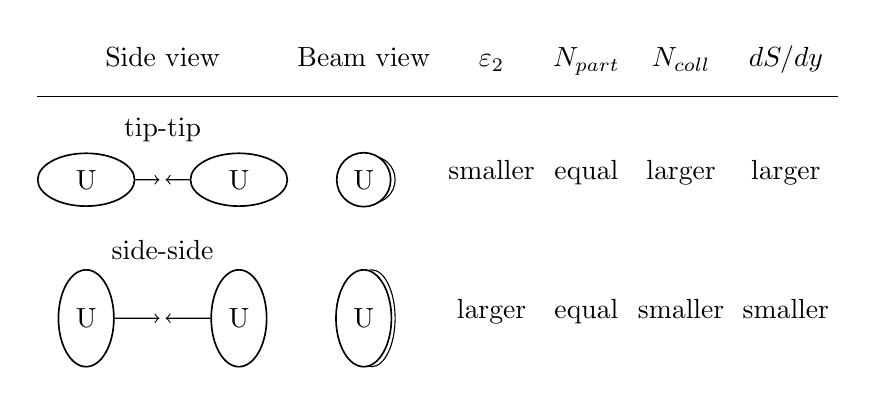
\begin{tikzpicture}[
    uranium/.style={draw, semithick, ellipse, anchor=center},
    small width/.style={minimum width=17},
    large width/.style={minimum width=35},
    small height/.style={minimum height=17},
    large height/.style={minimum height=35}
  ]
    \matrix (m) [matrix of nodes] {
      &[-5mm] Side view &[-5mm] & Beam view & $\varepsilon_2$ & $N_\text{part}$ & $N_\text{coll}$ & $dS/dy$ \\[1ex]
      \hline \\[1ex]
      & tip-tip & & & & & & \\
      |[uranium, large width, small height] (ttl)| U & &
      |[uranium, large width, small height] (ttr)| U &
      \node[draw, circle, small height, small width, xshift=1mm] {};
      \node[uranium, circle, small width, small height, fill=white] {U}; &
      smaller & equal & larger & larger \\[2ex]
      & side-side & & & & & \\
      |[uranium, large height, small width] (ssl)| U & &
      |[uranium, large height, small width] (ssr)| U &
      \node[draw, ellipse, large height, small width, xshift=1mm] {};
      \node[uranium, large height, small width, fill=white] {U}; &
      larger & equal & smaller & smaller \\
    };
    \begin{scope}[->]
      \draw (ttl) -- ($(ttl)!.48!(ttr)$);
      \draw (ttr) -- ($(ttr)!.48!(ttl)$);
      \draw (ssl) -- ($(ssl)!.48!(ssr)$);
      \draw (ssr) -- ($(ssr)!.48!(ssl)$);
    \end{scope}
  \end{tikzpicture}
\end{figure}
\end{frame}

%%%%%%%%%%%%%%%%%%%%%%%%%%%%%%%%%%%%%%%%%%%%%%%%%%%%%%%%%%%%%%%%%%%%%%%%%%%%%%%%%%%%%%%%%%%%%%%%%%%%%%%%%
\begin{frame}{Results: Uranium-Uranium collisions}
  \begin{itemize}
   \item Binary collisions: predict steep, negative slope of $v_2$ with increasing multiplicity (dashed line) in U+U, slight rise predicted in Au+Au
   \vspace{0.1 in}
   \item Data (symbols and solid line) no such trend! Slopes of U+U and Au+Au similar.
  \end{itemize}
  \vspace{0.2 in}
  \centering
  \includegraphics[width=0.8\columnwidth]{UU_Glb} \\
  \footnotesize STAR: H. Wang et al.:arXiv:1406.7522
\end{frame}

\begin{frame}{Results: Uranium-Uranium collisions}
  \begin{itemize}
   \item {\trento}: U+U tip-tip collisions same as side-side. Generalized mean is homogenous.
  \end{itemize}
  \begin{center}
   \includegraphics[width=0.5\columnwidth]{UU_homog-crop}
  \end{center}
  
  \begin{textblock*}{0.5\textwidth}(2.65cm,0cm)
   $4\,M(p; 1,1) = M(p; 4,4)$
  \end{textblock*}
  \vspace{0.3 in}
  \hrule
  \centering
  \vspace{0.1 in}
  \includegraphics[width=0.8\columnwidth]{uranium_trento}
\end{frame}


%%%%%%%%%%%%%%%%%%%%%%%%%%%%%%%%%%%%%%%%%%%%%%%%%%%%%%%%%%%%%%%%%%%%%%%%%%%%%%%%%%%%%%%%%%%%%%%%%%%%%%%
\begin{frame}{Summary}
\begin{itemize}
 \item Hybrid models using hydro + Boltzmann cascade: \\ powerful tool to extract QGP medium properties from data 
 \vspace{0.1 in}
 \item Of existing initial condition models, only IP-Glasma is able to describe flow harmonics in heavy-ion collisions. However,
       It does a poor job describing small collision systems such as p+p and p+Pb
 \vspace{0.1 in}
 \item Introduce {\trento} an effective, flexible model for initial conditions based on carefully chosen ansatz for entropy deposition
 \vspace{0.1 in}
 \item Will embed {\trento} in systematic model-to-data comparison to extract optimal value of nuissance parameter $p$ and
       place tighter constraints on QGP shear viscosity $\eta/s$
\end{itemize}
 
\end{frame}


%%%%%%%%%%%%%%%%%%%%%%%%%%%%%%%%%%%%%%%%%%%%%%%%%%%%%%%%%%%%%%%%%%%%%%%%%%%%%%%%%%%%%%%%%%%%%%%%%
\begin{frame}[noframenumbering]
 \frametitle{RHIC and LHC see signals of new state of matter}
 \centering
 \includegraphics[width=0.45\columnwidth]{thermal_RHIC}
 \hspace{0.05 in}
 \includegraphics[width=0.45\columnwidth]{thermal_LHC}\\
 \vspace{-0.1 in}
 \scriptsize Andronic, Braun-Munzinger, Redlich, Stachel, Nucl. Phys. A904-905 (2013)
 \normalsize \vspace{0.1 in}
 \begin{itemize}
  \item Particle yields well described by statistical hadronizaton models at a fixed temperature $T_c \sim 165$ MeV from $0.2-2.76$ TeV!
  \item Suggests all particles created from thermal source at fixed temp.
  \item Transition temperature in excellent agreement with lattice QCD!
 \end{itemize}
 
\end{frame}

%%%%%%%%%%%%%%%%%%%%%%%%%%%%%%%%%%%%%%%%%%%%%%%%%%%%%%%%%%%%%%%%%%%%%%%%%%%%%%%%%%%%%%%%%%%
\begin{frame}{Viscous relativistic hydrodynamics}
 Stress-energy tensor 
 \begin{equation*}
  T^{\mu\nu} = T^{\mu\nu}_\text{ideal} + \pi^{\mu\nu}
 \end{equation*}
 Ideal part 
 \begin{equation*}
  T^{\mu\nu}_\text{ideal} = (e+P)u^\mu u^\nu - P g^{\mu\nu}
 \end{equation*}
 Shear viscous correction
 \vspace{-0.1 in}
 \begin{eqnarray*}
  \cr \pi^{\mu\nu} &=& \eta \nabla^{\langle \mu} u^{\nu \rangle} \\
  \nabla^{\langle \mu} u^{\nu \rangle} &=& \nabla^\mu u^\nu + \nabla^\nu u^\mu - \tfrac{2}{3} \Delta^{\mu\nu} \nabla_\alpha u^\alpha
 \end{eqnarray*}
 Orthogonal projector
 \begin{equation}
  \Delta^{\mu\nu} = g^{\mu\nu} - u^\mu u^\nu
 \end{equation}

\end{frame}

%%%%%%%%%%%%%%%%%%%%%%%%%%%%%%%%%%%%%%%%%%%%%%%%%%%%%%%%%%%%%%%%%%%%%%%%%%%%%%%%%%%%%%%%%%%%%%%%
\begin{frame}[noframenumbering]{Initial condition models: Color-Glass Condensate theory}
 
\begin{itemize}
 \item Gluons dominate low-x nucleon content at high energies (DIS)
 \item Gluons of fixed energy (hence size) will eventually tightly pack nucleon
 \item Can only add more gluons by packing smaller wavelengths (recursive)
 \item $Q_s$ defines saturation momentum \emph{at given momentum fraction x}
\end{itemize}
\vspace{0.2 in}
e.g. Kharzeev-Levin-Nardi (KLN) model \\
$\frac{dN_g}{d^2r_\perp dy} = \frac{4 N_c}{N_c^2-1} \int\limits^{p_\perp^\text{max}} \frac{d^2p_\perp}{p^2_\perp} \int\limits^{p_\perp} \frac{d^2k_\perp}{4} \alpha_s(Q_s^2) \, \phi_A(x_1,p_1; {\bf r}_\perp) \, \phi_B(x_2,p_2; {\bf r}_\perp)$ \\
\vspace{0.1 in}
where $~~\phi(x,k_\perp; {\bf r}_\perp) \sim \frac{1}{\alpha_s(Q_s^2)} \frac{Q_s^2}{\max(Q_s^2,k^2_\perp)}$\\
\vspace{0.2 in}
KLN model reduces to approximate analytic form \\
\vspace{0.05 in}
$\frac{dN_g}{d^2r_\perp dy} \sim T_\text{min} (2+\log(T_\text{max}/T_\text{min}))$

\end{frame}

\end{document}
title
